\documentclass[tikz]{standalone}
\usetikzlibrary{decorations.pathmorphing}
\tikzset{snake it/.style={decorate, decoration=snake}}

\begin{document}
	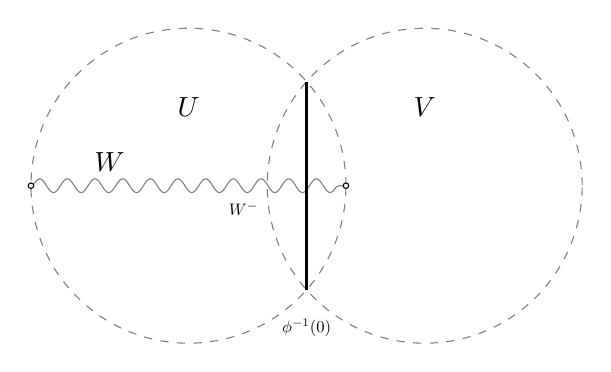
\begin{tikzpicture}
	\draw[gray, dashed] (0,0) circle (2);
	\node at (0,1){$U$};
	\draw[gray, dashed] (3,0) circle (2);
	\node at (3,1){$V$};
	\draw[gray, snake it] (-2,0) -- (2,0);
	\draw[black, fill=white] (-2,0) circle (1pt);
	\draw[black, fill=white] (2,0) circle (1pt);
	\draw[thick] (1.5, 1.32) -- (1.5, -1.32);
	\node[scale=.6] at (1.5, -1.8){$\phi^{-1}(0)$};
	\node[scale=.6] at (.7, -.3){$W^-$};
	\node[scale=1] at (-1, .3){$W$};
	\end{tikzpicture}
\end{document}